{\chapter{Background}}
\label{sec:background}

\section{Organic Semiconductors}

Semiconducting properties of conjugated polymers built by alternating electron donor and acceptor moieties \cite{mattinenAtomicLayerDeposition2021}, 


\subsection{Electronic Structure}

Since inorganic semiconductors' band theory does not take into consideration the Coulomb and exchange electron-electron interaction, which play a major role in organic semiconductors, it is necessary to add new theoretical approaches. On one hand, the transport properties are better described in terms of a hopping mechanism and the optoelectronic properties are better described by the molecular orbital picture \cite{alcacerElectronicStructureOrganic2018}. Since the device under study in this work is a transistor and their transport properties in aqueous and quasi-solid environments, the theoretical approach used will be the hopping mechanism.

\subsection{Molecular Doping}

Use of small molecules
Electron-deficient dopants such as 2,3,5,6 tetrafluoro-7,7,8,8-tetracyanoquinodimethane (F$_{4}$TCNQ) extract electrons from shallow HOMO p-type OMIECs, increasing hole concentration \cite{tanOrganicMixedIonic2022}.

\subsubsection{Measuring techniques to characterize doping}

\section{Organic Mixed Ionic/Electronic Conductors (OMIECs)}

Initially investigated for batteries and super capacitors, where the induction of charges was the main objective of a semiconducting material, OMIECs has rapidly grown to include other applications, among them: OECTs \cite{paulsenOrganicMixedIonic2020}.

% PEDOT:PSS Heterogeneous, blends or complexed systems OMIEC. Conjugated polymer/electrolyte blends. Contains ions chemically linked ot an insulating or conjugated component
% p(g3T2-T) Homogeneous, single-component systems OMIEC. Conjugated polymer electrolytes. Ions introduced as free species upon material casting or device operation

Commonly semiconducting polymers which are redox-active and can simultaneously conduct ions and electrons. Electronic charges accumulated on the conjugated polymer backbone result in secondary property changes in electrochemical potential and electronic conductivity, allowing OMIECs to be implemented in a variety of devices such as chemical sensors, organic electrochemical transistors, and energy storage electrodes \cite{tanOrganicMixedIonic2022}.

\subsection{A widely used material: PEDOT:PSS}
%\subsection{Engineering of semiconducting polymers}
Due to its commercial availability, operational stability, and relatively high performance, the conductive polymer poly(3,4-ethylenedioxythiophene) poly(styrene-sulfonate) (PEDOT:PSS) became a standard material for p-type OECTs. Its main drawback lays in its depletion-mode operation, which requires a voltage to turn off the device (as represented in Figure 1(b)). With the aim of minimizing power consumption, there is a special interest to design semiconducting polymers that would allow accumulation-mode devices (Figure 1(c)) with high performance \cite{nielsenMolecularDesignSemiconducting2016} \cite{tanOrganicMixedIonic2022}.

\subsection{Other Thiophene-based polymers}
%Seria chevere tener un grafico de como thiophene publications empezaron a crecer.
Thiophene is a planar conjugated ring structure consists of six delocalized pi-electrons. The aromatic nature arises from the four pi electrons and one unshared lone pair of electrons of the oxygen as six delocalized pi-electrons. It folow Hucke´s rule. Hene it is aromatic compound

Nielsen et al. reported a series of semiconducting polymers with Ethylene Glycol (EG) side chains designed to elucidate important strcuture-property guidelines for accumulation-mode OECT operation. They demonstrated that an OECT with 3-(2-(2-(2-methoxyethoxy)ethoxy)ethoxy)thiophene p(g3T2-T), as seen in Figure , has higher transconductance, and a turn-on voltage close to zero compared to other thiophene-based species \cite{nielsenMolecularDesignSemiconducting2016}. While its backbone design warrant reversibility during electrochemical redox reactions and good electronic transport, the EG side chains enable its stability in aqueous electrolytes and efficient transport of ionic and electronic charge carrier \cite{moiaDesignEvaluationConjugated2019}. Moser et al. studied the impact of the length of the EG side chain of this polythiophene backbone on the performance of OECTs. They reported that reducing chain length would maximize the capacitance, but the increase of length would enhance ion-polymer interaction. Finally, they suggested an optimum length of 3 monomers in side chains over 2, 4 and 6 monomers \cite{moserEthyleneGlycolBasedSide2020}. The main advantage of p(g3T2-T) over PEDOT:PSS is its higher transconductance \cite{nielsenMolecularDesignSemiconducting2016}, the absence of extensive pre- and postprocessing to optimize polymer stability and electrochemical performance in aqueous media and the possibility of an accumulation-mode OECT with low operation voltages\cite{moserEthyleneGlycolBasedSide2020}.

Organic semiconductors with polar sidechains have been identified as a promising class of materials for the field of bioelectronics. These materials, also called organic mixed ionic/electronic conductors (OMIECs), can exchange ions with aqueous electrolytes when electronic charge carriers are injected, transported, and stored in the bulk of the material \cite{giovannittiEnergeticControlRedoxActive2020}

Homogeneous single phase OMIECs (types V and VI) display larger magnitudes of ionic–electronic coupling and larger values of volumetric capacitance than biphasic OMIECs (types I–IV) \cite{paulsenOrganicMixedIonic2020}. 


%actually from reference 44, benchmarking omiecs for transistors

\subsection{Electrochemical Doping}

The electrochemical charging of OMIECs can be described as a capacitive faradaic charging process,
% there is current caused by charge transfer, other physical phenomenas such as desorption or adsorption can also lead to the aparition of current that is non faradaic reaction
meaning that the OMIEC undergoes a change in its oxidation state (p-doping in the language of physicists) through an electron transfer with the contact (current collector), while ions from the electrolyte penetrate inside the channel material to compensate the carge carrier on the polymer backbone electrostatically with no change in the inserted ion's oxidation state \cite{giovannittiEnergeticControlRedoxActive2020}  

Savva et al. study the influence of water on the performance of OECT, the water uptake of conjugated polymer films led to 10-13\% mass increase under non biased conditions. As the concentration of water decrease (NaCl$_{aq}$ 10 mM, 100mM, 1M, and 6M) ionic charging is faster regardless of the doping pulse, however the fastest ionic charging is achieved at NaCl$_{aq}$ 1 M. The injection/drift of ions is also affected by the ion-counterion attractive forces which delays the ion injection from the electrolyte, opposing their drift into the polymer (NaCl$_{aq}$ 6 M hinders the drift of anions) affecting the response time. \cite{savvaInfluenceWaterPerformance2019}

\section{Organic Electrochemical Transistors (OECTs)}

Organic Electrochemical Transistors (OECTs) consists of metallic source, drain and gate electrodes, an organic semiconductor channel (specifically an OMIEC as described in previous section) and an electrolyte that couples channel and gate \cite{rivnayOrganicElectrochemicalTransistors2018}

\begin{figure}[ht]
	\centering
	\subfloat[]{{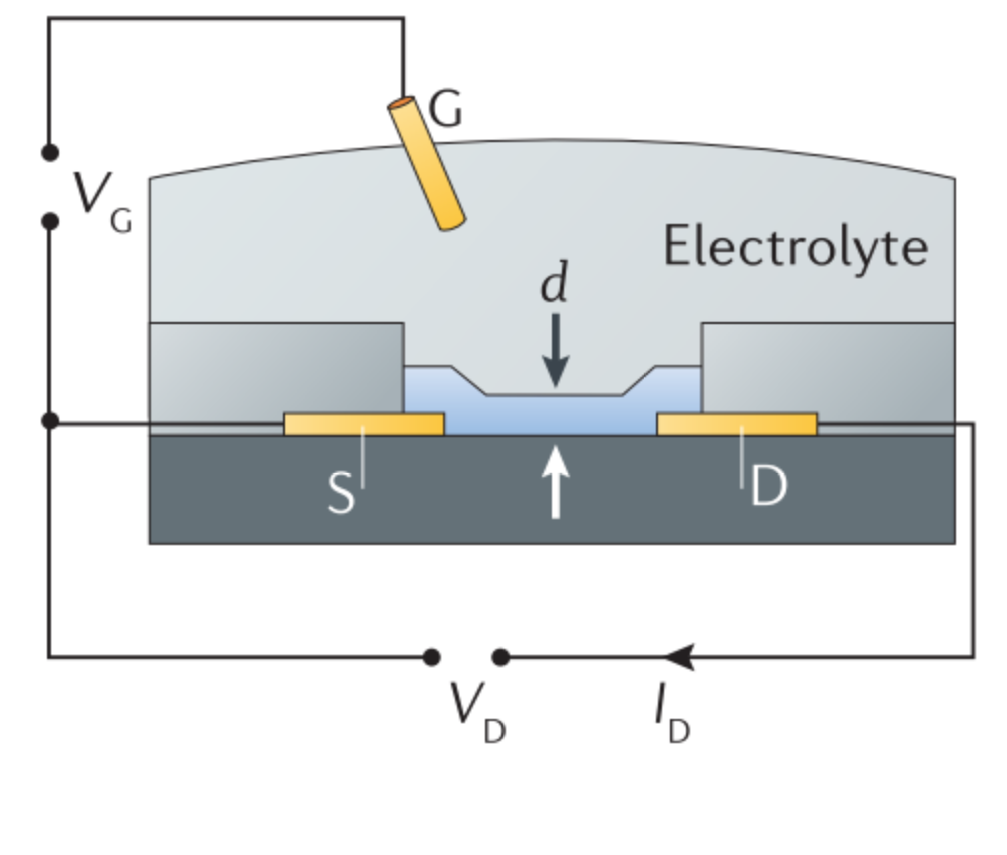
\includegraphics[height=4.5cm]{Images/structure.png} }}
	\qquad
	\subfloat[]{{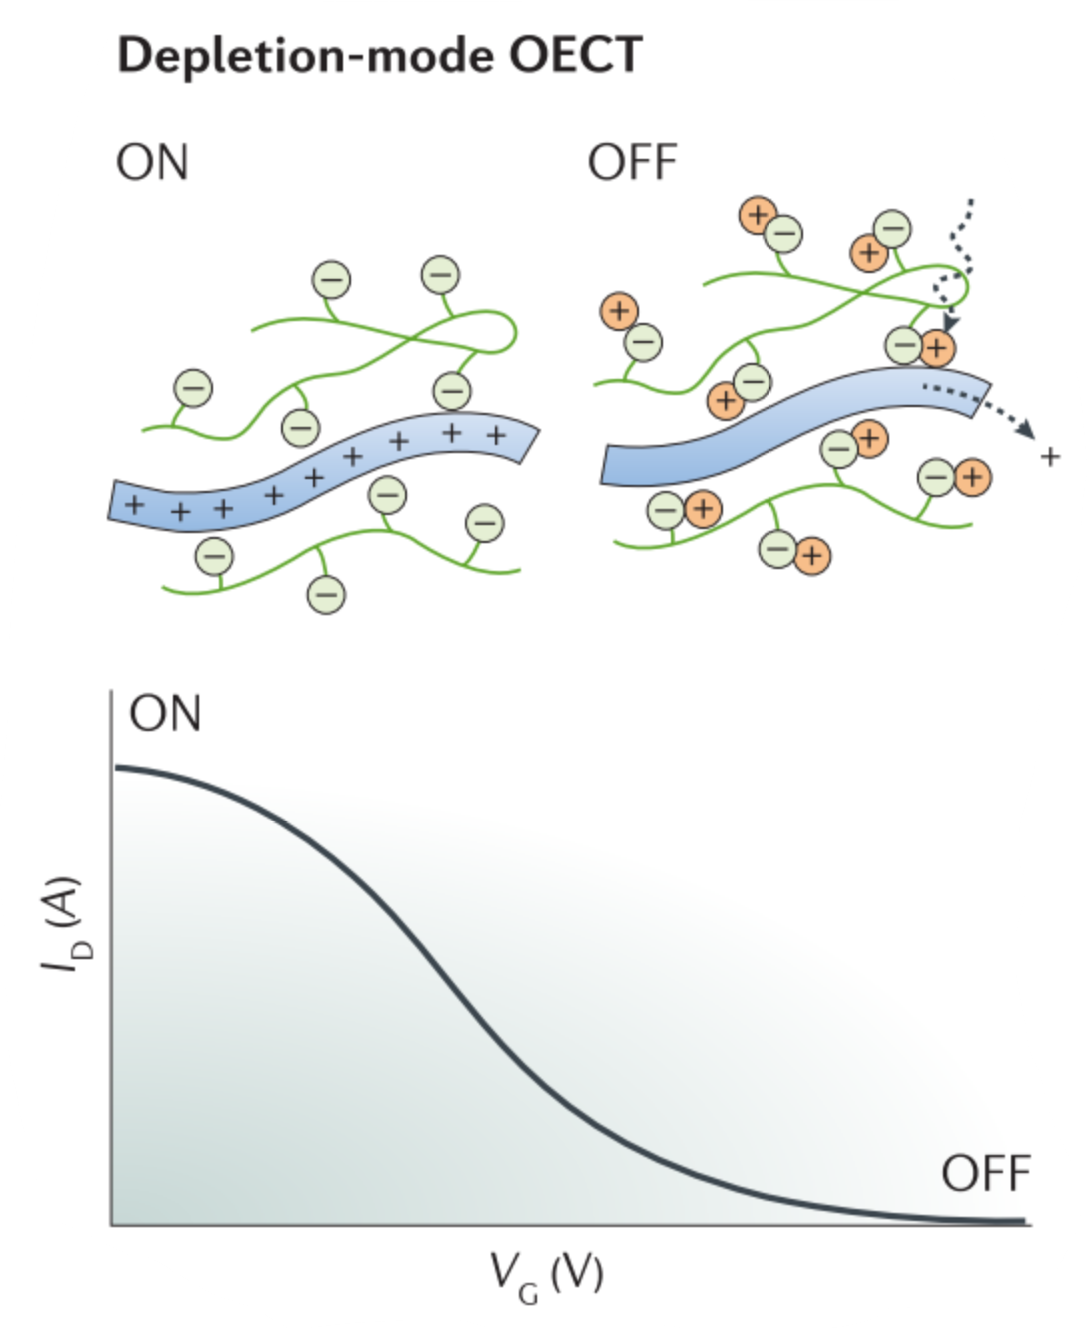
\includegraphics[height=8cm]{Images/depletion.png} }}
	\subfloat[]{{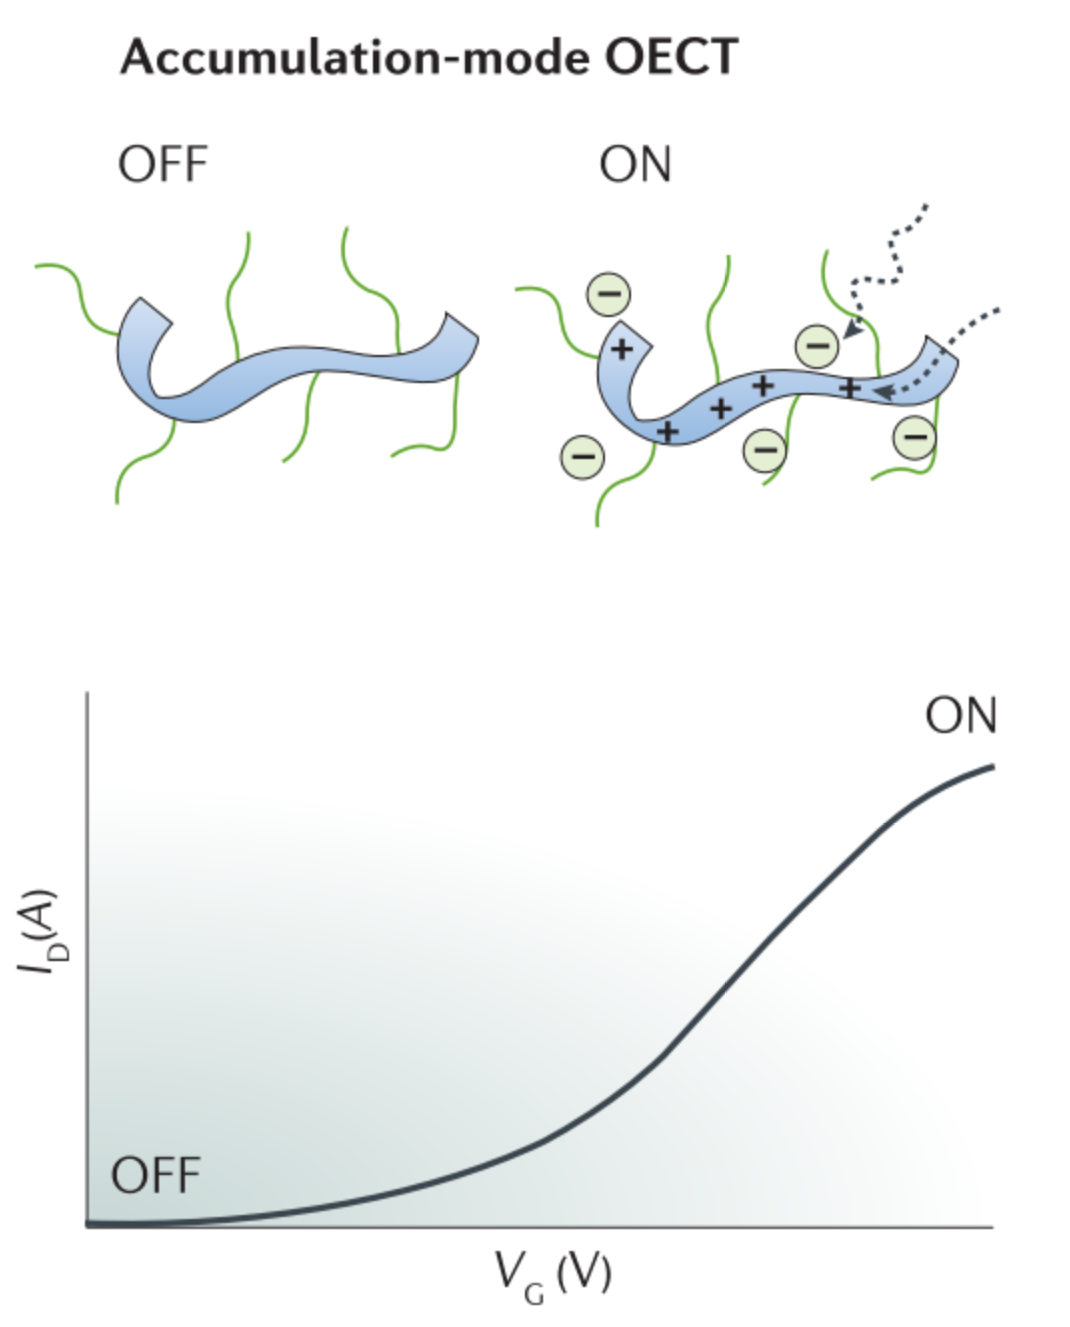
\includegraphics[height=8cm]{Images/accumulation.png} }}
	\caption{(a) Typical structure of an organic electrochemical transistor (OECT). (b) Transfer curve showing depletion-mode operation of an OECT with a conducting polymer channel. (c) Transfer curve showing accumulation-mode operation of an OECT with a semiconducting polymer channel. Images extracted from reference \cite{rivnayOrganicElectrochemicalTransistors2018}.}
	\label{fig:modes}
\end{figure}

The semiconductor

%devices that are mechanically compliant, biocompatible, and are sensitive to biochemical modules \cite{tanMixedIonicElectronic2022} 

\subsection{Device Physics}

\subsection{Operation Modes}

Accumulation-mode devices has the advantage of dissipating less static power when the device is not operated, due to low OFF current, which must be minimized as much as possible \cite{giovannittiEnergeticControlRedoxActive2020}

\subsection{Important Figures of Merit}
\subsubsection{Transconductance}
\subsubsection{$\mu$C* product}
\subsubsection{Threshold voltage}

An approach to shift the operating voltage range for PEDOT:PSS OECTs to lower the channel current, leading to reduced power consumption, is to tune the threshold voltage by de-doping PEDOT:PSS using commercially available amine-based molecular de-dopants \cite{Keene_enhmod_pedot}. Tan et al., on the other hand, explored a different approach, rather than modifying the doping level of the channel, they tuned the doping level of the gate to shift the threshold voltage. They used p(g3T2-T) and obtained a 400mV change with 60\% mol ratio of 2,3,5,6-Tetrafluoro-7,7,8,8-tetracyanoquinodimethane (F4TCNQ) dopant. The advantage over this approach is i) protecting the material from oxidation, since the Fermi level in brought towards the highest occupied molecular orbital (HOMO), and ii) no interference with the channel which helps to leave the transconductance unaffected \cite{tanTuningOrganicElectrochemical2022}.

\subsection{Requirements to Avoid Undesirable Side Reactions}


Achieving effective charge transfer between the analyte and OMIEC requires appropriate alignment of the electrochemical potential of electrons on the OMIEC electrode and the redox specie. Failure to do so may result in the subsequent transfer of charges to other redox-active sinks in the environment, leading to undesirable side reactions and products that may interfere with the OMIEC’s operation. Electrons flow from a region of higher to lower electrochemical potential. Hence, achieving electron transfer from redox-active species to the OMIEC requires the latter to have a deep LUMO (high electron affinity) \cite{tanMixedIonicElectronic2022} %paper

\subsubsection{Oxygen Reduction Reaction (ORR)}

With the aim of developing accumulation-mode OECTs, the engineering of new OMIECs were introduced as commented in previous sections. Normally, this polymer backbones have low ionization potential (IPs) which lead to another side effect issue that little attention has been paid: non capacitive faradaic rections in ambient: electron-transfer reaction from the OMIEC to molecular oxygen described as oxygen reduction reaction (ORR)

% Remember 
% Thermodynamically favored processes or reactions are those that involve both a decrease in the internal energy of the components (ΔH° < 0) and an increase in entropy of the components (ΔS° > 0). These processes are necessarily “thermodynamically favored” (ΔG° < 0) or negative. ΔG° = ΔH°-TΔS°
% Catalyst help to reduce the activation energy required for a reaction

The ORR yields either H$_{2}$O$_{2}$ or water (H$_{2}$O) as well as charging (oxidation) of the OMIEC that acts as the catalyst. The first shows a free energy difference that is endergonic for OMIECs with IPs \> 4.9eV and hence prevent the OMIEC from undergoing ORR that form H$_{2}$O$_{2}$. To prevent the ORR in ambient conditions, OMIECs based on donor-acceptor copolymer (Type III or IV) that have large IPs to shift
\cite{giovannittiEnergeticControlRedoxActive2020}
% Actually this material does not avoid this, we need to take into account this interaction.

\subsection{Building Block for neuromorphic and bioelectronic applications}



%%% Local Variables: 
%%% mode: latex
%%% TeX-master: "thesis"
%%% End: 
